\documentclass[]{article}

\usepackage[top=1in, bottom=1.25in, left=0.9in, right=0.9in]{geometry}
\usepackage{titlesec}
\titleformat{\section}
  {\normalfont\Large}
  {\thesection}{1em}{}
\titleformat{\subsection}
  {\normalfont\large}
  {\thesection}{1em}{}
\usepackage{wallpaper}
\usepackage{color}
\usepackage{xcolor}
\usepackage{hyperref}
\definecolor{blue}{rgb}{0.01, 0.28, 1.0}
\definecolor{lightgray}{rgb}{0.95, 0.95, 0.95}
\hypersetup{colorlinks=true, urlcolor=blue, citecolor=blue, filecolor=blue, linkcolor=blue}
\makeatletter
\renewcommand{\maketitle}{\bgroup\setlength{\parindent}{0pt}
\begin{flushleft}
	\begin{center}
 	\huge{\@title}\vspace{0.5cm}\\
	\quad\Large Bruno Vandekerkhove\vspace{0.5cm}\\
  	\qquad\large\textit{\@author}
	\end{center}
\end{flushleft}\egroup
}
\makeatother
\newcommand{\fakesection}[1]{
	\section*{#1}
	\par\refstepcounter{section}
	\addcontentsline{toc}{section}{#1}
}
\newcommand{\fakesubsection}[1]{
	\subsection*{#1}
	\par\refstepcounter{subsection}
	\addcontentsline{toc}{subsection}{\protect\numberline{\thesubsection}#1}
}
\newcommand{\parx}{\par\noindent}
\usepackage{tikz}
\usepackage[cachedir=minted]{minted}
\usepackage[cachedir=minted]{minted}
\usepackage{wallpaper}

\makeatletter
\renewcommand\tableofcontents{%
    \@starttoc{toc}%
}
\makeatother

\begin{document}

\thispagestyle{empty}

\title{Modelling of Complex Systems}
% \author{Bruno Vandekerkhove}
\date{}
\maketitle

%\tableofcontents

\begin{figure}[h]
\centering
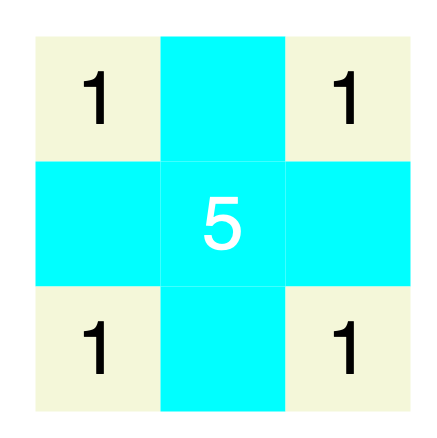
\includegraphics[width=0.2\textwidth]{img/error}
\caption{Nurikabe error in my theory (others got it right).}
\end{figure}

\fakesection{IDP Project}

None of us used auxiliary functions. These make the model solutions faster and can also make rules more readable.

\fakesubsection{Light Up}

We all had about the same solution except Afraz who didn't use aggregation which lead to more constraints. Our approach seemed reasonable even if it deviated from the model solution.

\fakesubsection{Train Tickets}

I think I'm the only one who didn't 'optimise' the solutions, and we came to the conclusion that the assignment wasn't all that clear about that (I made a thread on the discussion forum but not everybody read Simon's answer). I think my \texttt{halt($s_1$,$s_2$)} constrained was a bit cluttered. It could have been more readable by using convenience functions. I thought of using a simple reachability relationship but I preferred my approach at the time because it's easier to extend. I also forgot to impose that pass - and stop numbers start at zero. Not sure about the others in that respect.\\

\par\noindent I also want to note that my theory outputs 256 models, not 160. I don't know if that's actually a mistake (I asked a question on the discussion board just a few minutes ago.).

\fakesubsection{Nurikabe}

We had very similar solutions, I forgot the constraint that a numbered cell needs to contain land (\textit{`each numbered cell is a land cell'}) and made a toy example on which my theory fails (see above). The others did have this constraint as far as I could tell. Adapting the rule that says that every island needs to consist of the right number of land cells would solve this, and it's really just a matter of adding `$\land\ land(p)$' at the end.

\fakesubsection{Conclusion}

The feedback was relaxed and somewhat useful. There was not that much to mention because of the similarity of our solutions. If someone had a large number of rules it was hard to discuss his solution live since it takes a while to figure out what each rule is supposed to mean. In my opinion providing model solutions was enough feedback in and of itself (it's fairly easy to compare), but this only took an hour and may be worth re-doing next year. I can't speak for the others.

% 
% References
%
%\bibliographystyle{plain}
%\bibliography{references}
%\addcontentsline{toc}{section}{References}

\end{document}